\subsubsection{Map}
\label{sssec:map}

\paragraph{Resumen} Esta función {\tt map}, se distribuye automáticamente sobre el sistema
distribuido, y puede trabajar ya sobre {\it chunks} (partición) de datos
que se encuentran dentro de los diferentes nodos, a los cuales se les distribuye el
procesamiento de dicha función. 

\begin{figure}[h!]
  \centering
  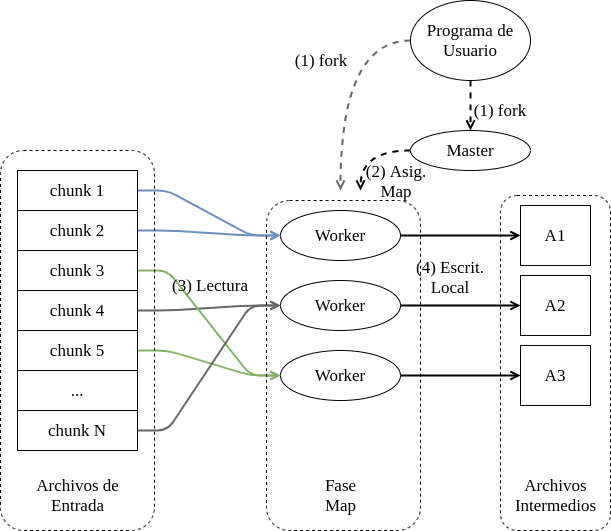
\includegraphics[width=0.75\linewidth]{figuras/MapReduce_mapper_phase.png}
  \caption{MapReduce: Fase {\tt map}}
  \label{fig:mapreduce_mapper_phase}
\end{figure}



\begin{enumerate}
\item {\bf fork:} El sistema distribuido se encarga de realizar la replicación
      de la aplicación del usuario sobre el conjunto de máquinas, esta
      aplicación se divide en copias que son {\it workers} y una especial que
      se denomina {\it master}\footnote{Esto es análogo a lo que se estudia en
      la cátedra con OpenMPI.}. Este último es el encargado de dividir las
      tareas a las copias que son workers.
\item {\bf Asig. Map:} El {\it master} asigna las tareas a los workers. Los
      cuales, cabe aclarar, trabajan sobre un o varios chunks de datos locales al
      nodo.
\item {\bf Lectura:} Un {\it worker} al que se le asigna una tarea {\tt map},
      lee los contenidos de los {\it archivos de entrada}, interpreta estos
      datos en formato clave-valor y se encarga de distribuir estos pares a la
      función {map}. Los valores que se produzcan por la función {\it map}, 
      se almacenan en un buffer de memoria.
\item {\bf Escritura Local:} Periodicamente, los pares que se almacenan en el
      buffer de memoria, pasan a ser escritos al disco de manera particionada. Las 
      ubicaciones de las particiones se comunican al {\it master} el cual será
      responsable más adelante de distribuir esta info. a los {\it workers} que
      son parte del {\it reduce}.
\end{enumerate}
